\documentclass[a4paper]{article}
\usepackage{hyperref}
\usepackage{xcolor}
\usepackage{graphicx}
\usepackage{float}
\usepackage[export]{adjustbox}
\usepackage[english]{babel}
\usepackage[T1]{fontenc}
\usepackage{url}
\usepackage{import}
\usepackage{multirow}
\usepackage{color}
\usepackage{fancyhdr}
\usepackage{amssymb}
\usepackage{tabu}
\usepackage{mathtools}
\usepackage[margin=2.5cm]{geometry}
\usepackage{listings}
\usepackage{titling}
\usepackage{listingsutf8}
\usepackage[utf8]{inputenc}
\usepackage[numbered,framed]{matlab-prettifier}
\usepackage{amsmath}
\usepackage{animate}
\usepackage[labelformat=empty]{caption}
\usepackage{subfig}
\usepackage{numprint}
\usepackage{parskip}

\DeclareUnicodeCharacter{2212}{}

\setlength{\parindent}{0pt}

\let\ph\mlplaceholder
\lstMakeShortInline"

\newcommand{\bnb}{\begin{nobreak}}
\newcommand{\enb}{\end{nobreak}}

\lstset{
	style              = Matlab-editor,
  	basicstyle         = \mlttfamily,
  	escapechar         = ",
  	mlshowsectionrules = true,
}

\pretitle{
	\begin{center}
  		\LARGE
  		
\includegraphics[width=\textwidth/4]{assets/logo-unifi.png}\\[\bigskipamount]
}
\posttitle{\end{center}}

\title{\vspace{2cm}Elaborato di\\ \textbf{Calcolo Numerico}\\ Anno Accademico 2018/2019\vspace{1cm}}

\author
{Alessio Falai - \texttt{6134275} alessio.falai@stud.unifi.it\\Leonardo Calbi - \texttt{6155786} leonardo.calbi@stud.unifi.it}

\date{}

\addto\captionsenglish{\renewcommand{\contentsname}{Capitoli}}

\begin{document}

\pagenumbering{Roman}
\lstset{inputencoding=latin1}
	
\maketitle

\begin{center}
	\today{}
\end{center}

\newpage

\newpage

\tableofcontents
\newpage

\pagenumbering{arabic}

\section{\textbf{Capitolo 1}}
\subsection{Esercizio 1}
Verificare che, per $h$ sufficientemente piccolo:
	\[
		\frac{3}{2} f(x) - 2f(x-h) + \frac{1}{2} f(x-2h)= hf'(x) + O(h^3)
	\]

\hspace{1cm}
\par\noindent\rule{\textwidth}{0.4pt}
\hspace{1cm}

Usando gli sviluppi di Taylor fino al secondo ordine otteniamo:
	\[
	f(x) = f(x_\mathrm{0}) + f'(x_\mathrm{0})h + \frac{1}{2} f''(x_\mathrm{0})h^{2} + O(h^3)
	\]
	\[
	f(x-h) = f(x_\mathrm{0}) + f'(x_\mathrm{0})(x-h-x_\mathrm{0}) + \frac{1}{2} f''(x_\mathrm{0})(x-h-x_\mathrm{0})^{2} + O(h^3)
	\]
	\[
	f(x-2h) = f(x_\mathrm{0}) + f'(x_\mathrm{0})(x-2h-x_\mathrm{0}) + \frac{1}{2} f''(x_\mathrm{0})(x-2h-x_\mathrm{0})^{2} + O(h^3)
	\]
Dato che $x-x_\mathrm{0}=h$, ponendo $x_\mathrm{0}=x-h$, si ha che:
	\[
	f(x-h)=f(x_\mathrm{0})+ O(h^3)
	\]
	\[
	f(x-2h) = f(x_\mathrm{0}) - f'(x_\mathrm{0})h + \frac{1}{2} f''(x_\mathrm{0})h^{2} + O(h^3)
	\]
Effettuando le opportune sostituzioni, la relazione iniziale diventa:
	\[
	\frac{3}{2}f(x_\mathrm{0}) + \frac{3}{2}f'(x_\mathrm{0})h + \frac{3}{4} f''(x_\mathrm{0})h^{2} - 2f(x_\mathrm{0}) + \frac{1}{2}f(x_\mathrm{0}) - \frac{1}{2}f'(x_\mathrm{0})h + \frac{1}{4} f''(x_\mathrm{0})h^{2} + O(h^3)=hf'(x) + O(h^3)
	\]
Semplificando, si ottiene che:
	\[
	f'(x_\mathrm{0})h+f''(x_\mathrm{0})h^{2}+O(h^3)=hf'(x) + O(h^3)
	\]
A questo punto, scriviamo lo sviluppo di Taylor anche per $f'(x)$:
	\[
	f'(x) = f'(x_\mathrm{0}) + f''(x_\mathrm{0})h + O(h^2)
	\]
Infine, otteniamo che:
	\[
	f'(x_\mathrm{0})h+f''(x_\mathrm{0})h^{2}+O(h^3)=f'(x_\mathrm{0})h + f''(x_\mathrm{0})h^{2} + O(h^3)
	\]
Dunque, l'uguaglianza iniziale è verificata.

\newpage
\subsection{Esercizio 2}
Quanti sono i numeri di macchina normalizzati della doppia precisione IEEE? Argomentare la risposta.

\hspace*{\fill}
\par\noindent\rule{\textwidth}{0.4pt}
\hspace*{\fill}

Nella doppia precisione IEEE si utilizzano 64 bit per rappresentare un numero in virgola mobile in macchina.
Di questi, il primo bit è riservato al segno $\pm$, i 52 bit successivi rappresentano la mantissa $\rho$ e i restanti 11 l'esponente $\eta$.
Un numero reale può essere rappresentato in macchina mediante la formula $r=\pm \rho \eta$, con $\rho=\sum_{i=1}^{m} \alpha_\mathrm{i}b^{1-i}$ e $\eta=b^{e-\nu}$.
Nel caso dei numeri normalizzati, abbiamo delle restrizioni sui numeri rappresentabili in macchina:
\begin{itemize}
	\item La mantissa è assunta della forma $1.f$ 
	\item Lo shift $\nu$ è pari a 1023
	\item Il valore $e$ deve essere compreso tra 0 e 2047, estremi esclusi
\end{itemize}
Dunque, per ricavare il numero di numeri normalizzati della doppia precisione IEEE, contiamo le possibili combinazioni di bit, date le condizioni sopra definite:
\begin{itemize}
	\item Per il segno abbiamo solo due possibilità, $+$ oppure $-$
	\item Per la mantissa abbiamo esattamente $2^{52}$ opzioni
	\item Per il valore di $e$ abbiamo esattamente 2046 opzioni
\end{itemize}
Dato che lo shift $\nu$ non cambia il numero di combinazioni possibili, moltiplicando i dati sopra ottenuti si ottiene:
$$2\times2^{52}\times2046=2^{53}\times2046=\numprint{18428729675200069632}$$

\newpage
\subsection{Esercizio 3}
Eseguire il seguente $script$ Matlab:
\begin{lstlisting}[caption = {}]
	format long e
	n=75;
	u=1e-300;for i=1:n,u=u*2;end,for i=1:n,u=u/2;end,u
	u=1e-300;for i=1:n,u=u/2;end,for i=1:n,u=u*2;end,u
\end{lstlisting}
Spiegare i risultati ottenuti.

\hspace*{\fill}
\par\noindent\rule{\textwidth}{0.4pt}
\hspace*{\fill}

L'obiettivo del programma proposto è verificare, dopo una serie di operazioni, che il numero restituito sia uguale a quello di partenza e
che quindi non si abbia perdita di informazione.

\underline{Alcune premesse}:

In caso di underflow, ovvero quando un calcolo produce un valore più piccolo di $realmin$, in accordo con l’opzione dello standard IEEE,
in Matlab i numeri vengono denormalizzati, perdono quindi il primo 1 sottinteso e sono definiti dalla loro rappresentazione binaria.
Inoltre, il più piccolo numero positivo denormalizzato è $\numprint{0.494}\times10^{-323}$. Ogni risultato più piccolo di questo è posto a zero.

\underline{Alcune notazioni importanti}:
\begin{itemize}
	\item $realmin$ è il minimo numero normalizzato rappresentabile in Matlab
	\item $realmax$ è il massimo numero normalizzato rappresentabile in Matlab
	\item $eps$ è la precisione di macchina
\end{itemize}

\underline{I risultati ottenuti}:
\begin{lstlisting}[caption = {}]
u =
	1.000000000000000e-300

u =
	1.119916342203863e-300
\end{lstlisting}

Prima di tutto viene impostato il formato di output a $longE$, formato long decimal (15 cifre dopo la virgola) con notazione scientifica.
Dopodichè, i primi 2 for effettuano prima 75 moltiplicazioni per 2 del numero $u$ e poi lo stesso numero di divisioni per 2 di $u$,
mantenendone il valore al di sopra di $realmin$ e facendo sì che non ci sia perdita di informazione (underflow).
I for successivi invece, a causa dello svolgersi prima delle 75 divisioni e poi delle 75 moltiplicazioni, portano alla denormalizzazione del numero e
quindi a una sua approssimazione, che risulta nel valore finale di $u$.

\newpage
\subsection{Esercizio 4}
Eseguire le seguenti istruzioni Matlab:
\begin{lstlisting}[caption = {}]
	format long e
	a=1.111111111111111
	b=1.11111111111111
	a+b
	a-b
\end{lstlisting}
Spiegare i risultati ottenuti.

\hspace{1cm}
\par\noindent\rule{\textwidth}{0.4pt}
\hspace{1cm}

I risultati ottenuti:
\begin{lstlisting}[caption = {}]
a =
	1.111111111111111e+00

b =
	1.111111111111110e+00

ans =
	2.222222222222221e+00

ans =
	8.881784197001252e-16

\end{lstlisting}

L'obiettivo del programma proposto è verificare se i risultati dati da operazioni di somma e sottrazione siano soggetti a cancellazione numerica o meno.\\

Innanzitutto, come nel precedente esercizio, viene impostato il formato di output a $longE$, formato long decimal (15 cifre dopo la virgola) con notazione scientifica.
Dopodichè, osservando gli output ottenuti, l'operazione di somma risulta ben condizionata, mentre l'operazione di sottrazione di due numeri 
molto vicini tra loro risulta invece mal condizionata.
Tale malcondizionamento deriva dal fatto che in macchina la semplice operazione $a-b$ viene effettuata come $fl(fl(a)-fl(b))$, dove con $fl(x)$ 
indichiamo il valore floating point del numero $x$.\\
Dunque, il numero $a-b = realmin + eps\times4$, mentre invece dovrebbe essere $10^{-15}$. Calcolando i vari valori floating, otteniamo:\\
$$fl(a) = \numprint{1.11111111111111093840975172498}$$\\
$$fl(b) = \numprint{1.11111111111111005023133202485}$$\\
$$fl(a) - fl(b) = \numprint{8.881784197001300}\times10^{-16}$$\\
$$fl(fl(a) - fl(b)) = \numprint{8.881784197001252}\times10^{-16}$$\\
Abbiamo così ricostruito l'output restituito da Matlab, che è frutto di una propagazione dell'errore relativa alla rappresentazione dei numeri decimali in macchina.

\newpage

\newpage
\section{\textbf{Capitolo 2}}
\subsection{Esercizio 5}
Scrivere $function$ Matlab distinte che implementino efficientemente
i seguenti metodi per la ricerca degli zeri di una funzione:
\begin{itemize}
	\item Metodo di bisezione;
	\item Metodo di Newton;
	\item Metodo delle secanti;
	\item Metodo delle corde.
\end{itemize}
Detta $x_\mathrm{i}$, l'approssimazione al passo $i$-esimo, utilizzare come criterio di arresto
$$|x_\mathrm{i+1} - x_\mathrm{i}| \leq tol\cdot(1+|x_\mathrm{i}|),$$
essendo $tol$ una opportuna tolleranza specificata in ingresso.

\hspace*{\fill}
\par\noindent\rule{\textwidth}{0.4pt}
\hspace*{\fill}

\textbf{Metodo di bisezione}:
\lstinputlisting[language=Matlab]{Chapter-2/Exercise-5/bisection.m}
\textbf{Metodo di Newton}:
\lstinputlisting[language=Matlab]{Chapter-2/Exercise-5/newton.m}
\begin{minipage}{\textwidth}
	\textbf{Metodo delle secanti}:
	\lstinputlisting[language=Matlab]{Chapter-2/Exercise-5/secant.m}
\end{minipage}
\begin{minipage}{\textwidth}
	\textbf{Metodo delle corde}:
	\lstinputlisting[language=Matlab]{Chapter-2/Exercise-5/chord.m}
\end{minipage}

\newpage
\subsection{Esercizio 6}
Utilizzare la $function$ del precedente esercizio per determinare un'approssimazione della
radice della funzione
$$f(x)=x-e^{-x}cos(\frac{x}{100}))$$
per $tol=10^{-i}, i=1,2,...,12$, partendo da $x_\mathrm{0}=-1$. Per il metodo di bisezione utilizzare 
$[-1,1]$, come intervallo di confidenza iniziale. Tabulare i risultati, in modo da confrontare le iterazioni
richieste da ciascun metodo. Commentare il relativo costo computazionale.

\hspace{1cm}
\par\noindent\rule{\textwidth}{0.4pt}
\hspace{1cm}

\begin{lstlisting}[language=Matlab, caption=Codice Matlab]
	f = @(x) x - exp(-x) * cos(x / 100);
	f1 = @(x) 1 + exp(-x) * cos(x / 100) + (exp(-x) * sin(x / 100)) / 100;
	x0 = -1;
	a = -1;
	b = 1;
	imax = 1000;
	for i = 1 : 12
		tol = 10^(-i);
		rtol=['Tolleranza: ',num2str(tol, '%e')];
		disp(rtol)
		[xB, it] = bisection(f, a, b, tol);
		disp(['Bisezione: ', num2str(xB, '%10.12e'), ' Iterazioni ', num2str(it)])
		[xN, it] = newton(f, f1, x0, imax, tol);
		disp(['Newton: ', num2str(xN, '%10.12e'), ' Iterazioni ', num2str(it)])
		[xC, it] = chord(f, f1, x0, imax, tol);
		disp(['Corde: ', num2str(xC, '%10.12e'), ' Iterazioni ', num2str(it)])
		[xS, it] = secant(f, f1, x0, imax, tol);
		disp(['Secanti: ', num2str(xS, '%10.12e'), ' Iterazioni ', num2str(it)])
		disp(' ')
	end
\end{lstlisting}

\begin{table}[h]
\caption{Risultati}
\centering
\resizebox{\textwidth}{!}{%
\begin{tabular}{|c|c|c|c|c|c|c|c|c|}
\hline
& \multicolumn{2}{c|}{\textbf{Bisezione}} & \multicolumn{2}{c|}{\textbf{Newton}} & \multicolumn{2}{c|}{\textbf{Secanti}} & \multicolumn{2}{c|}{\textbf{Corde}} \\ \hline
Tolleranza & Risultato & Iterazioni & Risultato & Iterazioni & Risultato & Iterazioni & Risultato & Iterazioni \\ \hline
$10^{-1}$ & 5.000000000000e-01 & 3 & 5.663058026183e-01 & 2 & 5.662928457961e-01 & 3 & 4.021808606807e-01 & 3 \\ \hline
$10^{-2}$ & 5.625000000000e-01 & 6 & 5.671373451066e-01 & 3 & 5.671339926161e-01 & 4 & 5.495185718942e-01 & 7 \\ \hline
$10^{-3}$ & 5.664062500000e-01 & 10 & 5.671373451066e-01 & 3 & 5.671339926161e-01 & 4 & 5.651741531555e-01 & 11 \\ \hline
$10^{-4}$ & 5.671386718750e-01 & 14 & 5.671374702932e-01 & 4 & 5.671374697616e-01 & 5 & 5.670103627779e-01 & 16 \\ \hline
$10^{-5}$ & 5.671386718750e-01 & 14 & 5.671374702932e-01 & 4 & 5.671374697616e-01 & 5 & 5.671232371728e-01 & 20 \\ \hline
$10^{-6}$ & 5.671386718750e-01 & 14 & 5.671374702932e-01 & 4 & 5.671374702932e-01 & 6 & 5.671358764609e-01 & 24 \\ \hline
$10^{-7}$ & 5.671374797821e-01 & 24 & 5.671374702932e-01 & 4 & 5.671374702932e-01 & 6 & 5.671372918144e-01 & 28 \\ \hline
$10^{-8}$ & 5.671374797821e-01 & 24 & 5.671374702932e-01 & 5 & 5.671374702932e-01 & 6 & 5.671374503070e-01 & 32 \\ \hline
$10^{-9}$ & 5.671374704689e-01 & 31 & 5.671374702932e-01 & 5 & 5.671374702932e-01 & 6 & 5.671374689985e-01 & 37 \\ \hline
$10^{-10}$ & 5.671374702360e-01 & 34 & 5.671374702932e-01 & 5 & 5.671374702932e-01 & 7 & 5.671374701482e-01 & 41 \\ \hline
$10^{-11}$ & 5.671374702943e-01 & 36 & 5.671374702932e-01 & 5 & 5.671374702932e-01 & 7 & 5.671374702770e-01 & 45 \\ \hline
$10^{-12}$ & 5.671374702943e-01 & 36 & 5.671374702932e-01 & 5 & 5.671374702932e-01 & 7 & 5.671374702914e-01 & 49 \\ \hline
\end{tabular}%
}
\end{table}

Analizzando i risultati ottenuti, abbiamo verificato che i metodi di bisezione e corde impiegano
un numero considerevolmente maggiore di iterazioni rispetto ai metodi di Newton e secanti, a paritá di tolleranza utilizzata. 
Questo è dato dal fatto che i primi due hanno convergenza lineare, mentre i secondi due hanno convergenza quadratica.

\newpage
\subsection{Esercizio 7}
Calcolare la molteplicità della radice nulla della funzione
$$f(x)=x^{2}sin(x^{2}).$$
Confrontare, quindi, i metodi di Newton, Newton modificato, e di Aitken, per approssimarla per gli
stessi valori di $tol$ del precedente esercizio (ed utilizzando il medesimo criterio di arresto),
partendo da $x_\mathrm{0}=1$. Tabulare e commentare i risultati ottenuti.

\hspace*{\fill}
\par\noindent\rule{\textwidth}{0.4pt}
\hspace*{\fill}

\textbf{Metodo di Newton modificato}:
\lstinputlisting[language=Matlab]{Chapter-2/Exercise-7/modnewton.m}
\textbf{Metodo di accelerazione di Aitken}:
\lstinputlisting[language=Matlab]{Chapter-2/Exercise-7/aitken.m}

Dato che il metodo di Newton modificato richiede espressamente la molteplicità della radice 
della funzione in esame, andiamo a calcolarla:
$$x^{2}sin(x^{2})=0 \rightarrow x^{2}=0 \lor sin(x^{2})=0$$
Le radici del polinomio sono $0$ e $k\sqrt{\pi}$, con $k\in\mathbb{Z}$.
La molteplicità della radice $x=0$ è pari a 3, mentre quella della radice $x=k\sqrt{\pi}$ è pari a 1.
Dunque, nel nostro caso, per l'utilizzo del metodo di Newton modificato, inizializzeremo il valore $m$
relativo alla molteplicità a 3.

\begin{lstlisting}[language=Matlab, caption=Codice Matlab]
f = @(x) x^2 * sin(x^2);
f1 = @(x) 2 * x * (sin(x^2) + x^2 * cos(x^2));
x0 = 1;
imax = 1000;
m = 3;
for i = 1 : 12
	tol = 10^(-i);
	rtol=['Tolleranza: ', num2str(tol, '%e')];
	disp(rtol)
	[xN, it] = newton(f, f1, x0, imax, tol);
	disp(['Newton: ', num2str(xN, '%10.12e'), ' Iterazioni ', num2str(it)])
	[xNM, it] = modnewton(f, f1, x0, m, imax, tol);
	disp(['Newton Modificato: ', num2str(xNM, '%10.12e'), ' Iterazioni ', num2str(it)])
	[xA, it] = aitken(f, f1, x0, imax, tol);
	disp(['Aitken: ', num2str(xA, '%10.12e'), ' Iterazioni ', num2str(it)])
	disp(' ')
end
\end{lstlisting}

\begin{table}[H]
\caption{Risultati}
\centering
\resizebox{\textwidth}{!}{%
\begin{tabular}{|c|c|c|c|c|c|c|c|c|}
\hline
& \multicolumn{2}{c|}{\textbf{Newton}} & \multicolumn{2}{c|}{\textbf{Newton modificato}} & \multicolumn{2}{c|}{\textbf{Aitken}} \\ \hline
Tolleranza & Risultato & Iterazioni & Risultato & Iterazioni & Risultato & Iterazioni \\ \hline
$10^{-1}$ & 3.843178806071e-01 & 2 & 2.163225010255e-02 & 1 & 6.492908618812e-19 & 3\\ \hline
$10^{-2}$ & 2.880513930938e-02 & 11 & 1.352015482798e-03 & 3 & 6.492908618812e-19 & 3\\ \hline
$10^{-3}$ & 2.883766303035e-03 & 19 & 8.450096767474e-05 & 5 & 6.492908618812e-19 & 3\\ \hline
$10^{-4}$ & 2.887022508866e-04 & 27 & 2.112524191869e-05 & 6 & 0.000000000000e+00 & 4\\ \hline
$10^{-5}$ & 2.890282391460e-05 & 35 & 1.320327619918e-06 & 8 & 0.000000000000e+00 & 4\\ \hline
$10^{-6}$ & 2.893545954951e-06 & 43 & 3.300819049795e-07 & 9 & 0.000000000000e+00 & 4\\ \hline
$10^{-7}$ & 2.896813203496e-07 & 51 & 2.063011906122e-08 & 11 & 0.000000000000e+00 & 4\\ \hline
$10^{-8}$ & 2.900084141257e-08 & 59 & 1.289382441326e-09 & 13 & 0.000000000000e+00 & 4\\ \hline
$10^{-9}$ & 2.903358772398e-09 & 67 & 3.223456103315e-10 & 14 & 0.000000000000e+00 & 4\\ \hline
$10^{-10}$ & 2.906637101090e-10 & 75 & 2.014660064572e-11 & 16 & 0.000000000000e+00 & 4\\ \hline
$10^{-11}$ & 2.909919131508e-11 & 83 & 1.259162540357e-12 & 18 & 0.000000000000e+00 & 4\\ \hline
$10^{-12}$ & 2.913204867832e-12 & 91 & 3.147906350894e-13 & 19 & 0.000000000000e+00 & 4\\ \hline
\end{tabular}%
}
\end{table}

Analizzando i risultati ottenuti, abbiamo verificato che il metodo di Newton impiega
un numero considerevolmente maggiore di iterazioni rispetto ai metodi di Newton modificato e Aitken, a paritá di tolleranza utilizzata. 
Questo è dato dal fatto che il primo ha convergenza lineare (in caso di radici multiple), mentre i secondi due hanno convergenza quadratica.

\newpage

\newpage
\section{\textbf{Capitolo 3}}
\subsection{Esercizio 8}
Scrivere una $function$ Matlab che, data in ingresso una matrice $A$, restituisca una matrice, $LU$, che contenga l’informazione sui suoi fattori $L$ ed $U$, ed un vettore \textbf{p} contenente la relativa permutazione, della fattorizzazione $LU$ con $pivoting$ parziale di $A$:
$$function [LU,p] = palu(A)$$
Curare particolarmente la scrittura e l’efficienza della $function$.

\hspace*{\fill}
\par\noindent\rule{\textwidth}{0.4pt}
\hspace*{\fill}

\textbf{Fattorizzazione LU con pivoting parziale}:
\lstinputlisting[language=Matlab]{Chapter-3/Exercise-8/palu.m}

\subsection{Esercizio 9}
Scrivere una $function$ Matlab che, data in ingresso la matrice $LU$ ed il vettore \textbf{p} creati dalla $function$ del precedente esercizio, ed il termine noto del sistema lineare $A\textbf{x} = \textbf{b}$, ne calcoli la soluzione:
$$function x = lusolve(LU,p,b)$$
Curare particolarmente la scrittura e l’efficienza della $function$.

\hspace*{\fill}
\par\noindent\rule{\textwidth}{0.4pt}
\hspace*{\fill}

\textbf{Risoluzione di un sistema lineare, con matrice dei coefficienti fattorizzata LU con pivoting parziale}:
\lstinputlisting[language=Matlab]{Chapter-3/Exercise-9/palusolve.m}

\subsection{Esercizio 11}
Scrivere una $function$ Matlab che, data in ingresso una matrice $A\in\mathbb{R}^{m\times n}$, con $m \geq n = rank(A)$, restituisca una matrice, $QR$, che contenga l’informazione sui fattori $Q$ ed $R$ della fattorizzazione $QR$ di $A$:
$$function \ QR = myqr(A)$$
Curare particolarmente la scrittura e l’efficienza della $function$.

\hspace*{\fill}
\par\noindent\rule{\textwidth}{0.4pt}
\hspace*{\fill}

\textbf{Fattorizzazione QR}:
\lstinputlisting[language=Matlab]{Chapter-3/Exercise-11/myqr.m}

\subsection{Esercizio 12}
Scrivere una $function$ Matlab che, data in ingresso la matrice $QR$ creata dalla $function$ del precedente esercizio, ed il termine noto del sistema lineare $A\textbf{x} = \textbf{b}$, ne calcoli la soluzione nel senso dei minimi quadrati:
$$function \ x = qrsolve(QR,b)$$
Curare particolarmente la scrittura e l’efficienza della $function$.

\hspace{1cm}
\par\noindent\rule{\textwidth}{0.4pt}
\hspace{1cm}

\textbf{Risoluzione di un sistema lineare, con matrice dei coefficienti fattorizzata QR}:
\lstinputlisting[language=Matlab]{Chapter-3/Exercise-12/qrsolve.m}


\newpage
\section{\textbf{Capitolo 4}}
\subsection{Esercizio 14}
Scrivere un programma che implementi efficientemente il calcolo del polinomio interpolante su un insieme di ascisse distinte.

\hspace*{\fill}
\par\noindent\rule{\textwidth}{0.4pt}
\hspace*{\fill}

\begin{minipage}{\textwidth}
    \textbf{Polinomio interpolante di Lagrange}:
    \lstinputlisting[language=Matlab]{Chapter-4/Exercise-14/lagrange.m}
\end{minipage}
\begin{minipage}{\textwidth}
    \textbf{Polinomio interpolante di Newton}:
    \lstinputlisting[language=Matlab]{Chapter-4/Exercise-14/newton.m}
\end{minipage}

\subsection{Esercizio 15}
Scrivere un programma che implementi efficientemente il calcolo del polinomio interpolante di Hermite su un insieme di ascisse distinte.

\hspace*{\fill}
\par\noindent\rule{\textwidth}{0.4pt}
\hspace*{\fill}

\textbf{Polinomio interpolante di Hermite}:
\lstinputlisting[language=Matlab]{Chapter-4/Exercise-15/hermite.m}

\subsection{Esercizio 16}
Scrivere un programma che implementi efficientemente il calcolo di una spline cubica naturale interpolante su una partizione assegnata.

\hspace*{\fill}
\par\noindent\rule{\textwidth}{0.4pt}
\hspace*{\fill}

\textbf{Risoluzione di un sistema tridiagonale}:
\lstinputlisting[language=Matlab]{Chapter-4/Exercise-16/trid.m}
\textbf{Spline cubica naturale}:
\lstinputlisting[language=Matlab]{Chapter-4/Exercise-16/spline3.m}

\subsection{Esercizio 19}
Calcolare (numericamente) la costante di Lebesgue per i polinomi interpolanti di grado $n = 2, 4, 8, ... , 40$, sia sulle ascisse equidistanti che su quelle di Chebyshev (utilizzare 10001 punti equispaziati per valutare la funzione di Lebesgue). Graficare convenientemente i risultati ottenuti. Spiegare, quindi, i risultati ottenuti approssimando la funzione
$$f(x)=\frac{1}{1+x^{2}},x\in[−5,5]$$
utilizzando le ascisse equidistanti e di Chebyshev precedentemente menzionate (tabulare il massimo errore valutato su una griglia di 10001 punti equidistanti nell’intervallo [−5, 5]).

\hspace{1cm}
\par\noindent\rule{\textwidth}{0.4pt}
\hspace{1cm}

\textbf{Costante di Lebesgue}:
\lstinputlisting[language=Matlab]{Chapter-4/Exercise-19/lebesgue.m}
\textbf{Ascisse di Chebyshev}:
\lstinputlisting[language=Matlab]{Chapter-4/Exercise-19/ceby.m}

\begin{lstlisting}[language=Matlab, caption=Codice Matlab]
f = @(x) 1 ./ (1 + x.^2);
a = -5;
b = 5;
n = 2:2:40;
kxi = zeros(length(n), 1);
kci = zeros(length(n), 1);
x = linspace(a, b, 10001);

ax1 = subplot(2,1,1);
for i = 1 : length(n)
	xi = linspace(a, b, n(i) + 1);
	fxi = f(xi);
	yxi = lagrange(xi, fxi, x);
	plot(ax1, x, yxi)
	hold on
	kxi(i, 1) = lebesgue(xi);
end
legend('2','4','6','8','10','12','14','16','18','20','22','24','26','28','30','32','34','36','38','40')
hold off

ax2 = subplot(2,1,2);
for i = 1 : length(n)
	ci = ceby(n(i) + 1, a, b);
	fci = f(ci);
	yci = lagrange(ci, fci, x);
	plot(ax2, x, yci)
	hold on
	kci(i, 1) = lebesgue(ci);
end
legend('2','4','6','8','10','12','14','16','18','20','22','24','26','28','30','32','34','36','38','40')
hold off
\end{lstlisting}

Le seguenti figure mostrano il polinomio di \textit{Lagrange}, al variare del grado \textit{n} del polinomio con $n=2,4,6,8...40$, utilizzando ascisse equidistanti e ascisse di Chebyshev:
\begin{figure}[H]
	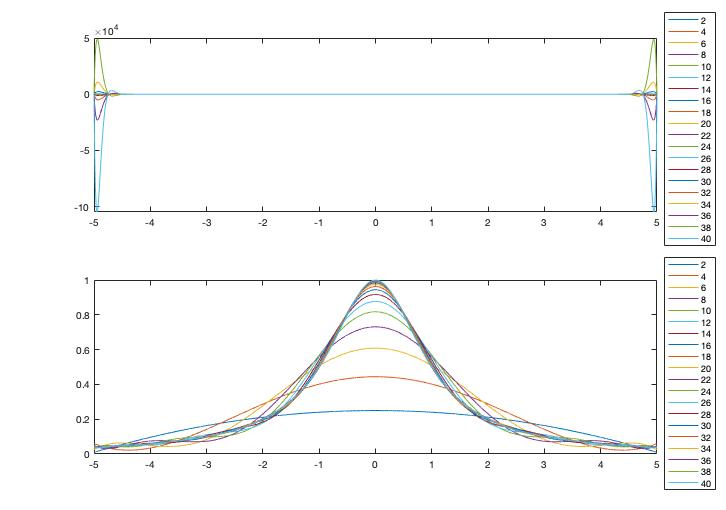
\includegraphics[width=\textwidth]{Chapter-4/Exercise-19/plot.jpg}
	\caption*{Polinomio di Lagrange con n° di ascisse $[2,4,6,8,..,40]$}
\end{figure}
Nelle seguenti tabelle è riportato come varia la \textit{costante di Lebesgue} $\Lambda$, al variare del grado \textit{n} del polinomio e si può notare come la crescita sia \textit{esponenziale}, per $n\rightarrow\infty$, prendendo in cosiderazione \textit{ascisse equidistanti}:\\\
\begin{table}
	\begin{center}
		\caption{Costante di Lebesgue con ascisse equispaziate}
		\begin{tabular}{|c|c|}
			\hline
			$n$ & $\Lambda$ \\
			\hline
			$2$  & $1.250000000000000$ \\ 
			$4$  & $2.207824277504000$ \\ 
			$6$  & $4.549341110838356$ \\ 
			$8$  & $10.945005461386041$ \\ 
			$10$ & $29.898141093562188$ \\ 
			$12$ & $89.323735973507041$ \\ 
			$14$ & $2.831809493441890e+02$ \\ 
			$16$ & $9.342736404823136e+02$ \\ 
			$18$ & $3.170339307979169e+03$ \\ 
			$20$ & $1.097924392398584e+04$ \\ 
			$22$ & $3.866684343844037e+04$ \\ 
			$24$ & $1.378514896760509e+05$ \\ 
			$26$ & $4.964824917524024e+05$ \\ 
			$28$ & $1.802445465492321e+06$ \\ 
			$30$ & $6.592504744423425e+06$ \\ 
			$32$ & $2.430870357380395e+07$ \\ 
			$34$ & $8.978560703086898e+07$ \\ 
			$36$ & $3.348225693891219e+08$ \\ 
			$38$ & $1.249687039228850e+09$ \\ 
			$40$ & $4.678649708006595e+09$ \\ 
			\hline
		\end{tabular}
	\end{center}
\end{table}
\begin{table}
	\begin{center}
		\caption{Costante di Lebesgue con ascisse di Chebyshev}
		\begin{tabular}{|c|c|}
			\hline
			$n$ & $\Lambda$ \\
			\hline
			$2$  & $1.429872254730518e+00$ \\ 
			$4$  & $1.685135237733246e+00$ \\ 
			$6$  & $1.866863755668355e+00$ \\ 
			$8$  & $2.008324271512492e+00$ \\ 
			$10$ & $2.123677735937467e+00$ \\ 
			$12$ & $2.221698051371436e+00$ \\ 
			$14$ & $2.304741888790266e+00$ \\ 
			$16$ & $2.381233643402699e+00$ \\ 
			$18$ & $2.447573290086530e+00$ \\ 
			$20$ & $2.508706712856935e+00$ \\ 
			$22$ & $2.549521672833381e+00$ \\ 
			$24$ & $2.612618302290017e+00$ \\ 
			$26$ & $2.647525891619366e+00$ \\ 
			$28$ & $2.699620139181539e+00$ \\ 
			$30$ & $2.742631723381937e+00$ \\ 
			$32$ & $2.771163414194285e+00$ \\ 
			$34$ & $2.802963771799375e+00$ \\ 
			$36$ & $2.839252073343268e+00$ \\ 
			$38$ & $2.869838999732480e+00$ \\ 
			$40$ & $2.909700595498265e+00$ \\ 
			\hline
		\end{tabular}
	\end{center}
\end{table}


\newpage
\section{\textbf{Capitolo 5}}
\subsection{Esercizio 22}
Scrivere due functions che implementino efficientemente le formule adattattive dei trapezi e di Simpson.

\hspace{1cm}
\par\noindent\rule{\textwidth}{0.4pt}
\hspace{1cm}

\textbf{Formule adattattive dei trapezi}:
\lstinputlisting[language=Matlab]{Chapter-5/Exercise-22/adaptrap.m}
\textbf{Formule adattattive di Simpson}:
\lstinputlisting[language=Matlab]{Chapter-5/Exercise-22/adapsimp.m}

\subsection{Esercizio 23}
Sapendo che $$I(f) = \int_{0}^{atan(30)} (1+tan^{2}(x))dx = 30, $$ tabulare il numero dei punti richiesti dalle formule adattative dei trapezi e di Simpson per approssimare $I(f)$, utilizzate con tolleranze $$ tol = 10^{-i}, i = 2,...,8,$$ assieme ai relativi errori.

\hspace*{\fill}
\par\noindent\rule{\textwidth}{0.4pt}
\hspace*{\fill}

\begin{lstlisting}[language=Matlab, caption=Codice Matlab]
f = @(x) 1 + tan(x)^2;
global pt;
global ps;
a = 0;
b = atan(30);
format long e;
for i = 2 : 8
    pt = 2;
    ps = 3;
    tol = 10^-i;
    I2 = adaptrap(f,a,b,tol);
    I4 = adapsimp(f,a,b,tol);
    pt
    et = abs(I2 - 30)
    ps
    es = abs(I4 - 30)
end
\end{lstlisting}

\begin{table}[H]
    \caption{Risultati}
    \centering
    \resizebox{\textwidth}{!}{%
    \begin{tabular}{|c|c|c|c|c|}
        \hline
            & \multicolumn{2}{c|}{\textbf{Trapezi}} & \multicolumn{2}{c|}{\textbf{Simpson}} \\ \hline
        Tolleranza & Punti & Errore & Punti & Errore \\ \hline
        $10^{-2}$ &  375 & 4.764530169460102e-03 & 49 & 2.372538178065042e-03 \\ \hline
        $10^{-3}$ & 1181 & 5.737280523554489e-04 & 77 & 6.165282965362451e-04 \\ \hline
        $10^{-4}$ & 3687 & 5.263954536971482e-05 & 137 & 5.016670867874495e-05 \\ \hline
        $10^{-5}$ & 11883 & 5.454611955002520e-06 & 249 & 2.220652294937508e-06 \\ \hline
        $10^{-6}$ & 37273 & 5.635538471437940e-07 & 425 & 3.981788339046943e-07 \\ \hline
        $10^{-7}$ & 116747 & 5.255170520968022e-08 & 765 & 3.565320128018357e-08 \\ \hline
        $10^{-8}$ & 375793 & 5.507661882120374e-09 & 1365 & 3.587672381399898e-09 \\ \hline
    \end{tabular}%
    }
\end{table}


\newpage
\section{\textbf{Capitolo 6}}
\subsection{Esercizio 24}
Scrivere una function che implementi efficientemente il metodo delle potenze.

\hspace{1cm}
\par\noindent\rule{\textwidth}{0.4pt}
\hspace{1cm}

\textbf{Metodo delle potenze}:
\lstinputlisting[language=Matlab]{Chapter-6/Exercise-24/power.m}

\newpage
\subsection{Esercizio 25}
Sia data la matrice di \textit{Toeplitz} simmetrica $$A_\mathrm{N}=\begin{pmatrix}
    4 & -1 & & -1 & & &\\
    -1 & \ddots & \ddots & & \ddots & \\
     & \ddots & \ddots &\ddots & & -1\\
     -1 & & \ddots & \ddots & \ddots & \\
     & \ddots & & \ddots & \ddots & -1 \\
     & & -1 & & -1 & 4
\end{pmatrix} \in\mathbb{R}^{NxN}, N\geq10, $$
in cui le extra-diagonali più esterne sono le none. Partendo dal vettore $\textbf{u}_\mathrm{0} = (1,...,1)^{T} \in \mathbb{R}^{N} $, applicare il metodo delle potenze con tolleranza $tol = 10^{-10}$ per $N = 10 : 10 : 500$, utilizzando la function del precedente esercizio. Graficare il valore dell'autovalore dominante, e del numero di iterazioni necessarie per soddisfare il criterio di arresto, rispetto ad $N$. Utilizzare la function \textbf{spdiags} di Matlab per creare la matrice e memorizzarla come matrice sparsa.

\hspace*{\fill}
\par\noindent\rule{\textwidth}{0.4pt}
\hspace*{\fill}
\begin{lstlisting}[language=Matlab, caption=Codice Matlab]
x = linspace(10, 500, 50);
ax1 = subplot(2, 1, 1);
ax2 = subplot(2, 1, 2);
l = zeros(50, 1);
it = zeros(50, 1);
tol = 1E-10;
for n = 10 : 10 : 500
     u = ones(n, 1);
     S = spdiags(u * [-1 -1 4 -1 -1], [-9, -1 : 1, 9], n, n);
     [l1, x1, i] = mypower(S, u, tol);
     l(n / 10) = l1;
     it(n / 10) = i;
end
plot(ax1, x, l);
plot(ax2, x, it);
legend(ax1, 'Autovalori dominanti');
legend(ax2, 'Iterazioni');
\end{lstlisting}
Le seguenti figure mostrano gli autovalori dominanti e le iterazioni necessarie al metodo delle potenze, al variare della dimensione della matrice  $A_\mathrm{N}$ con $N = 10 : 10 : 500$:
\begin{figure}[H]
     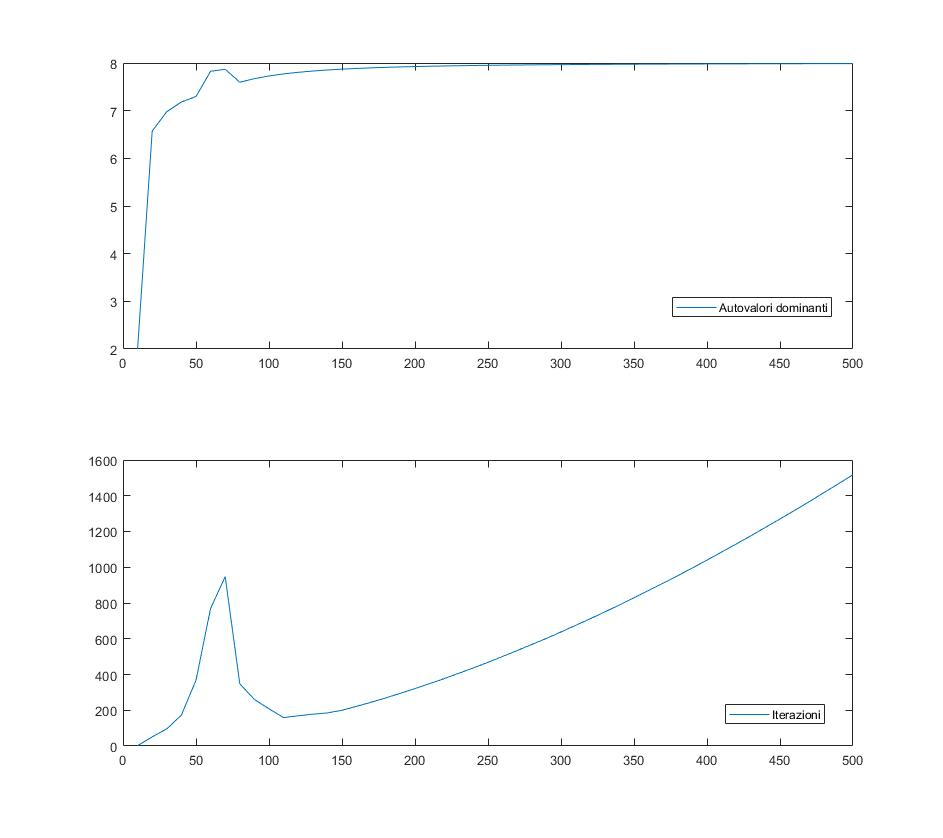
\includegraphics[width=\textwidth]{Chapter-6/Exercise-25/plot.jpg}
     \caption*{Autovalori dominanti e iterazioni del metodo delle potenze con $N = 10 : 10 : 500$}
\end{figure}

\newpage
\subsection{Esercizio 26}
Scrivere una function che implementi efficientemente un metodo iterativo, per risolvere un sistema lineare,
definito da un generico splitting della matrice dei coefficienti.

\hspace*{\fill}
\par\noindent\rule{\textwidth}{0.4pt}
\hspace*{\fill}

\begin{minipage}{\textwidth}
    \textbf{Risoluzione iterativa del sistema lineare definito dallo splitting A = M - N}:
    \lstinputlisting[language=Matlab]{Chapter-6/Exercise-26/itersolve.m}
\end{minipage}
\begin{minipage}{\textwidth}
    \textbf{Risoluzione iterativa del sistema lineare con il metodo msolve}:
    \lstinputlisting[language=Matlab]{Chapter-6/Exercise-26/gsplit.m}
\end{minipage}
\begin{minipage}{\textwidth}
    \textbf{Risoluzione iterativa del sistema lineare con il metodo msolve e matvec}:
    \lstinputlisting[language=Matlab]{Chapter-6/Exercise-26/asplit.m}
\end{minipage}

\newpage
\subsection{Esercizio 27}
Scrivere le function ausiliarie, per la function del precedente esercizio, che implementano i metodi
iterativi di Jacobi e Gauss-Seidel.

\hspace*{\fill}
\par\noindent\rule{\textwidth}{0.4pt}
\hspace*{\fill}

\begin{minipage}{\textwidth}
\textbf{Metodo di Jacobi per la funzione \textit{itersolve}}:
    \lstinputlisting[language=Matlab]{Chapter-6/Exercise-27/iterjacobi.m}
    \textbf{Metodo di Gauss-Seidel per la funzione \textit{itersolve}}:
    \lstinputlisting[language=Matlab]{Chapter-6/Exercise-27/itergs.m}
\end{minipage}
\begin{minipage}{\textwidth}
    \textbf{Metodo di Jacobi per la funzione \textit{gsplit}}:
    \lstinputlisting[language=Matlab]{Chapter-6/Exercise-27/jacobi.m}
    \textbf{Metodo di Gauss-Seidel per la funzione \textit{gsplit}}:
    \lstinputlisting[language=Matlab]{Chapter-6/Exercise-27/gs.m}
\end{minipage}

\newpage
\subsection{Esercizio 28}
Con riferimento alla matrice $A_\mathrm{N}$ definita in (1), risolvere il sistema lineare $$A_\mathrm{N}\textbf{x} = \begin{pmatrix}1 \\ \vdots \\ 1\end{pmatrix} \in\mathbb{R}^{N}, $$
con i metodi di Jacobi e Gauss-Seidel, per $N = 10 : 10 : 500$, partendo dalla approssimazione nulla della soluzione, ed imponendo che la norma del residuo sia minore di $10^{-8}$. Utilizzare, a tal fine, la function dell'esercizio 26, scrivendo function ausiliarie \textit{ad hoc} (vedi esercizio 27) che sfruttino convenientemente la struttura di sparsità (nota) della matrice $A_\mathrm{N}$. Graficare il numero delle iterazioni richieste dai due metodi iterativi, rispetto ad $N$, per soddisfare il criterio di arresto prefissato.
\hspace*{\fill}
\par\noindent\rule{\textwidth}{0.4pt}
\hspace*{\fill}

\textbf{Prodotto \textit{ad hoc} matrice vettore}:
\lstinputlisting[language=Matlab]{Chapter-6/Exercise-28/matvec.m}
\textbf{Metodo di Jacobi}:
\lstinputlisting[language=Matlab]{Chapter-6/Exercise-28/jacobi.m}
\textbf{Metodo di Gauss-Seidel}:
\lstinputlisting[language=Matlab]{Chapter-6/Exercise-28/gs.m}
\begin{lstlisting}[language=Matlab, caption=Codice Matlab]
x = linspace(10, 500, 50);
tol = 1E - 8;
ij = zeros(50, 1);
igs = zeros(50, 1);
for n = 10 : 10 : 500
    b = ones(n, 1);
    x0 = zeros(n, 1);
    [x, i] = splitting(b, @matvec, @jacobi, x0, tol);
    ij(n / 10) = i;
    [x, i] = splitting(b, @matvec, @gs, x0, tol);
    igs(n / 10) = i;
end
plot(x, ij, x, igs);
legend('Jacobi', 'Gauss-Seidel');
\end{lstlisting}
La seguente figura mostra il confronto del numero di iterazioni necessarie ai metodi di \textit{Jacobi} e \textit{Gauss-Seidel}, al variare della dimensione della matrice  $A_\mathrm{N}$ con $N = 10 : 10 : 500$:
\begin{figure}[H]
	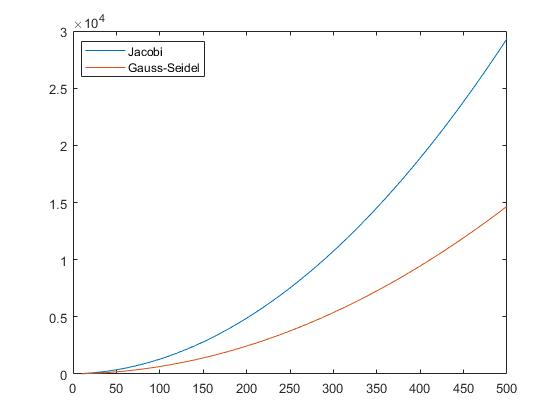
\includegraphics[width=\textwidth]{Chapter-6/Exercise-28/plot.jpg}
	\caption*{Numero iterazioni dei metodi di \textit{Jacobi} e \textit{Gauss-Seidel} con $N = 10 : 10 : 500$}
\end{figure}

\newpage

\newpage
\end{document}
